\documentclass[abstract=on,10pt,twocolumn]{scrartcl}

\usepackage{ucs}
\usepackage[utf8x]{inputenc}
\usepackage[T1]{fontenc}
\usepackage[english]{babel}
\usepackage{datetime}

\usepackage[paper=a4paper,top=2cm,left=1.5cm,right=1.5cm,bottom=2cm,foot=1cm]{geometry}

\usepackage{relsize}%	relative font sizes

\usepackage[retainorgcmds]{IEEEtrantools}%	IEEEeqnarray
\setlength{\IEEEnormaljot}{4\IEEEnormaljot}

\usepackage{indentfirst}
\usepackage[colorlinks=true,linkcolor=black,citecolor=black]{hyperref}
\usepackage{cleveref}
\usepackage{color}

\usepackage{todonotes}
\usepackage{hyperref}
\usepackage{cleveref}
\usepackage[cmex10]{amsmath}
\usepackage{epstopdf}
\usepackage{graphicx}
\usepackage{listings}

\usepackage{xspace}
\newcommand{\intel}{Intel\textsuperscript{\textregistered}\xspace}
\newcommand{\xeon}{Xeon\textsuperscript{\textregistered}\xspace}

\lstset{
	language=C++,
	basicstyle=\ttfamily,
	showspaces=false,
	showtabs=false,
	tabsize=3,
	captionpos=b,
	breaklines=true,
	breakatwhitespace=true
}


%%%%%%%%%%%%%%%%
%  title page  %
%%%%%%%%%%%%%%%%
\titlehead{University of Minho \hfill Master's Degree in Informatics Engineering\\Department of Informatics \hfill Computer Graphics - Integrated Project}

\title{Parallel Radix Sort}
%\subtitle{A Comparison of Shared Memory Parallel Libraries}

\author{
    \\Miguel Palhas\\
     	\texttt{\smaller pg19808@alunos.uminho.pt}
}

\date{Braga, \docdate}

%\subject{PAPI CUDA}

%%%%%%%%%%%
%  Hacks  %
%%%%%%%%%%%

%	Paragraph (title) with linebreak
\newcommand{\paragraphh}[1]{\paragraph{#1\hfill}\hfill

}

%	Add "Appendix" to the appendices titles, but not to the references
\usepackage{ifthen}
\newcommand*{\appendixmore}{%
  \renewcommand*{\othersectionlevelsformat}[1]{%
    \ifthenelse{\equal{##1}{section}}{\appendixname~}{}%
    \csname the##1\endcsname\autodot\enskip}
  \renewcommand*{\sectionmarkformat}{%
    \appendixname~\thesection\autodot\enskip}
}

\newdateformat{mmmyyyydate}{\monthname[\THEMONTH] \THEYEAR}
\newcommand{\docdate}{\mmmyyyydate\today}

\newcommand{\tm}{\textsuperscript{\texttrademark}}
\newcommand{\tr}{\textsuperscript{\textregistered}}

\newcommand{\todonaps}{\todo[inline,color=green!40]}

\begin{document}
	\maketitle

	\begin{abstract}
Following a previous work where some parallelization libraries were studied, a follow-up is shown in this document, by presenting an comparative analysis with the initial shared memory approach, with OpenMP, against Threading Building Blocks. More than to obtain performance gains, the goal is to analyse implementation details, studying what each library has to offer, and the difficulties it presents. The case study used for analysis is an implementation of the Radix Sort algorithm. 
\end{abstract}
	\section{Introduction}
\label{sec:100}

This document follows on a previous work where a sorting algorithm, in particular Radix Sort, was studied and parallelized in a shared memory approach with OpenMP, and a distributed memory approach with MPI. The follow-up is based on the shared memory implementation, which is now compared against a similar implementation using Intel\tr Threading Building Blocks.

\Cref{sec:200} shows a small description of the algorithm. More details on the algorithm and on previous implementations can be found in \cite{naps62sort}. The particular implementations are explained in \cref{sec:300,sec:400,sec:500}. In \cref{sec:600,sec:700}, methodology and testing environment are described, with some results being shown on \cref{sec:700}. Finally some conclusions are gathered on \cref{sec:900}. 
	\section{Radix Sort}
\label{sec:200}

Radix Sort is a non-comparative sorting algorithm that works on integer or string keys. The ordering is done by grouping keys into buckets, according to their individual digits.\\

The approach used here is the \emph{Least Significant Digit} one, which is iterative in nature, running through all the elements once for every digit


As a small example, consider the following list of integers:

\begin{lstlisting}
	arr = [170, 45, 75, 90, 24, 2, 66]
\end{lstlisting}

In the first iteration, the least significant digit is considered. After sending each key into the correct bucket, the result is the following:

\begin{lstlisting}
	0: [170, 90],
	2: [2],
	4: [24],
	5: [45, 75],
	6: [66]
\end{lstlisting}

And after merging all buckets:

\begin{lstlisting}
	arr = [170, 90, 2, 24, 45, 75, 66]
\end{lstlisting}

This completes the first iteration. The process is repeated until there are no more digits do process.
	\section{Sequential Approach}
\label{sec:300}

The initial implementation is straigh-forward, following the previously given explanation. There are some particularities however. Instead of base-10 digits, groups of bits were used. Each digit consists of a group of bits, allowing for better performance (with the usage of bitwise operators), and also giving the possibility of easily varying the digit size, which directly influences overall performance.

With a smaller amount of bits per digit, less buckets are created (number of buckets is $b=2^g$ where $g$ is the number of bits). Consequentely, more iterations will be necessary. On the other hand, a bigger value of $g$ will require more buckets, increasing data fragmentation and memory overhead.
	\section{OpenMP Implementation}
\label{sec:400}

For the OpenMP implementation used, 3 steps are required in each iteration:

\begin{enumerate}
	\item Bucket Fill
	\begin{itemize}
		\item[-] For $P$ threads and $B$ buckets, each thread will handle $B/P$ buckets
		\item[-] Each thread iterates entire array, inserting only on its own buckets
	\end{itemize}

	\item Master thread computes offset for each bucket on the result array

	\item Each thread copies its buckets to global array
\end{enumerate}

Given that radix sort is a non-comparative sorting algorithm, and it consists mostly on memory operations, it can be easily proven that it is completely memory bound. Because of that, no good results should be expected from this naive shared-memory implementation. The main bottleneck here is the fact that each thread iterates the array independently. Since each thread is not synchronized, no locality advantages will happen, and each thread will iterate at their own pace.

An alternative approach would be to iterate the array in smaller chuncks, synchronizing each thread after every chunck, to benefit from memory locality. However, because of time issues, and since the main goal of this work was not to obtain good results, but to study the implementation approaches, no effort was made in that direction.

	\section{Threading Building Blocks}
\label{sec:500}

Intel\tr developed the C++ Template Library Threading Building Blocks to offer a parallelization approach where the focus of the programmer could stay away from the parallelism intrinsic issues, and stay on the algorithm and \textit{useful} code.

The library attempts to provide an abstraction layer for the parallelism, effectively providing an almost completely different paradigm than the OpenMP library.

The most basic parallel operator in TBB is the \texttt{parallel\_for} function, which is the equivalent of \texttt{\#pragma omp parallel for} directive in OpenMP. This function takes as an argument a \textit{Functor}, or a class instance that defines the computation to be done in parallel.

TBB deals with the thread allocation and initialization, and also manages the workload, by dividing the range of iteration in chuncks. Each thread will receive a chunck that can be iterated just like a regular C++ collection. The \textit{Functor} allocated on that thread can then iterate through the chunck and perform the desired function, with full transparency from the threading and work assigning logic.

Besides the particular implementation details, the Radix Sort implementation follows a similar structure to the OpenMP implementation. Since Radix Sort consists mostly on array operations and iterations, there was no need for any TBB more complex operators like \texttt{parallel\_reduce} or \texttt{parallel\_pipeline}. However, the \texttt{concurrent\_vector} class proved useful for some specific issues that required the usage of explicit locks in the OpenMP version.

\subsection{TBB Paradigm}
It can be said that TBB, while providing excellent facilities to parallelize tasks and organize workload, also suffers from a couple of problems due to the paradigm it attempts to implement. Drawing much from functional paradigms, it requires the parallelizable logic to be encapsulated in a class object (namely, a \textit{Functor}). While this is good from a more abstract point of view, it also requires much more code to be written, for tasks that are sometimes rather simple. This issue might be solved with the usage of C++11 (recenlty known as C++0x), which allows the declaration of lambda functions. TBB supports this functions, allowing them to be passed as parameter to the parallelization directives, instead of an instance of a \textit{Functor}.

Another point that might provide some pitfalls to TBB is the complete abstraction of the threading model. While it is usually good to let the library handle all the background tasks of allocating threads and distribute the workload, this is not always the case. For most tasks it also possible to parameterize TBB functions, for example, with information about the desired granularity, which is useful to have some degree of control about the degree of division of the task.

It is not possible however, to have more low-level control over this. A particular example was found during the implementation of Radix Sort. Having each thread handling a set of buckets, with the index of those buckets being received as the chunck list to each thread, it was required to decide, for each element, wether or not the current thread was the one responsible for saving it. In OpenMP, this simply meant acquiring the thread id with the appropriate number, and decide from there if the destiny bucket was being handled by the current thread.
In TBB, however, there is no such thing as a thread id. This makes sense, but only to a certain extent, since it is TBB who decides how many threads are spawned. The only possible control over this is the maximum number of threads, but never the actual exact amount can be specified.
Because of this, the only way to determine if the bucket was assigned to the current thread was, for each element to insert, iterate over the entire chunck list, and check wether or not the index was there. This changed this computation from a simple bitwise operation and a comparison in OpenMP, to an entire loop in TBB.

Even though the chunck is probably small enough to eliminate any performance issues from this difference, the fact remains that the lack of a more controlable parallelization feature hurt this version.
	\section{Environmental Setup}
\label{sec:600}

All tests were run on the SeARCH cluster

All tests described in this document were performed using a very specific subset of nodes from the SeARCH\footnote{\url{http://search.di.uminho.pt}}, here referred as SeARCH Group Hex.
For each test, a single node was fully reserved, to ensure full access to all the resources.

Nodes in SeARCH Group Hex have two hex-core processors (with Intel\tr Hyper-threading\tm technology) and 12 to 48 GB of RAM.Further detail regarding the hardware of these nodes can be found in \cref{tab:grouphex}.


\begin{table}[!htp]
	\begin{center}
		\begin{tabular}{lc}
			\hline
			Processors per node: & 2	\\
			Processor model: & \intel\xeon X5650\\
			Cores per processor: & 6	\\
			Threads per core: & 2	\\
			Clock frequency: & 2.66 GHz	\\
			\hline
			L1 cache: & 32 KB + 32 KB per core	\\
			L2 cache: & 256 KB per core	\\
			L3 cache: & 12 MB shared	\\
			RAM: & 12 to 48 GB	\\
			\hline
		\end{tabular}
		\caption[SeARCH Group Hex hardware description]{SeARCH Group Hex hardware description. See \cite{xeon5600} for further detail about this processor.}
		\label{tab:grouphex}
	\end{center}
\end{table}
	\section{Test Methodology}
\label{sec:700}

All three versions of the algorithm analysed here (sequential, OpenMP and TBB) were tested and compared. For each version, 5 different input sizes were used, with all the input coming from the same randomly populated file, with over $2^{26}$ integer values. Digit size was also varied between 2 and 8 (although limitations in the OpenMP implementation only allowed it to be tested for 2, 4 and 8, and not the remaining values in the range).

For both parallel versions, the number of threads was also varied, between 2 and 32. Even though, as noted on \cref{sec:600}, the environment used has 12 cores per node, meaning a multiple of 12 should provide a better value for the number of threads, the OpenMP version had limitations, mostly due to the usage of bitwise operators to simplify bucket calculations, and could only work with a number of threads that was a power of 2.
	\section{Results}
\label{sec:800}

\Cref{fig:omp,fig:tbb} show the speedups measured for both the OpenMP and the TBB versions. As expected and explained in \cref{sec:400}, no speedups were expected, due to the extremely naive approach.

\begin{figure}[!htp]
	\centering
	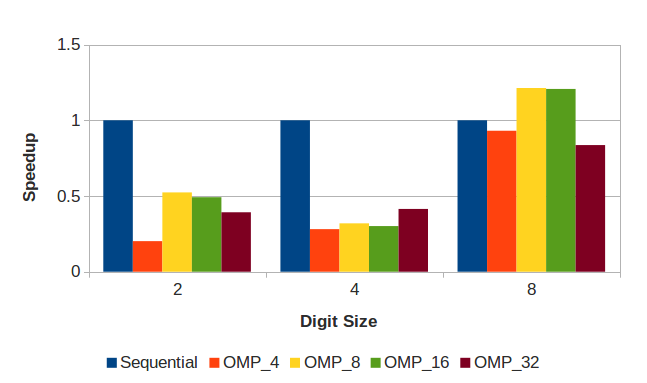
\includegraphics[width=\columnwidth]{plot-omp}
	\caption{Speedup results for OpenMP. Only the largest test case is shown}
	\label{fig:omp}
\end{figure}

OpenMP results show that speedups are only attained for 16 threads, with a digit size of 8 bits. However, a speedup of 1.2 with 16 threads is mostly insignificant, and it does not change the fact that the parallelization approach has problems.

\begin{figure}[!htp]
	\centering
	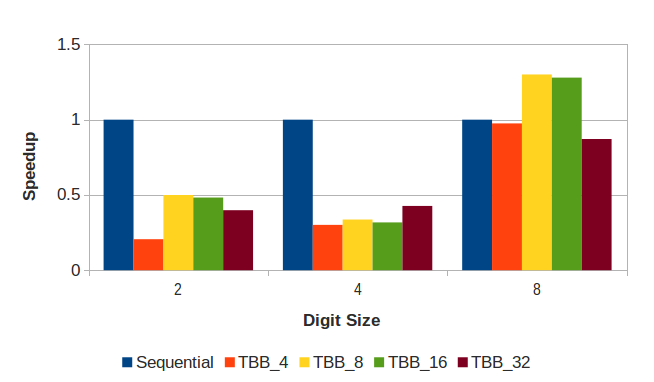
\includegraphics[width=\columnwidth]{plot-tbb}
	\caption{Speedup results for Threading Building Blocks. Only the largest test case is shown}
	\label{fig:tbb}
\end{figure}

Results for the equivalent tests on TBB show nearly the same values, with variatons not large enough to consider significant. This was expected since the parallelism approach did not change, only the underlying thread management library did, and if that would be a reason for significant performance differences, it would mean that the thread management of the slower one suffered from performance issues. This is not the case. Although particular overheads for library initialization and thread  spawning were not measured, total application time was measured, and did not show significant differences between OpenMP and TBB.

As for the results, it should also be noted that, even though no real performance gains can be achieved with the naive implementation, it can serve as a basis for a more robust approach, for example, using the suggested method of iterating by chuncks and synchronizing every thread between them. Also, results for 32 threads show an even worse performance decrease compared to other tests. This is due to the fact that 32 threads requires the node to try to take advantage of Hyper-Threading, which most of the cases ens up hurting performance, as can be seen by the results shown.

\subsection{OpenMP vs TBB}
\label{sec:810}

\Cref{fig:both-small,fig:both-big} show a comparison of the speedups achieved with both parallel implementations. Since the actual speedup is not demonstrative of the effectiveness of the libraries, because it is limited by the naive implementation, this serves to show that, from the two implementations, which are as much similar as it could be possible when using two different libraries, TBB seems to provide better results.

\begin{figure}[!htp]
	\centering
	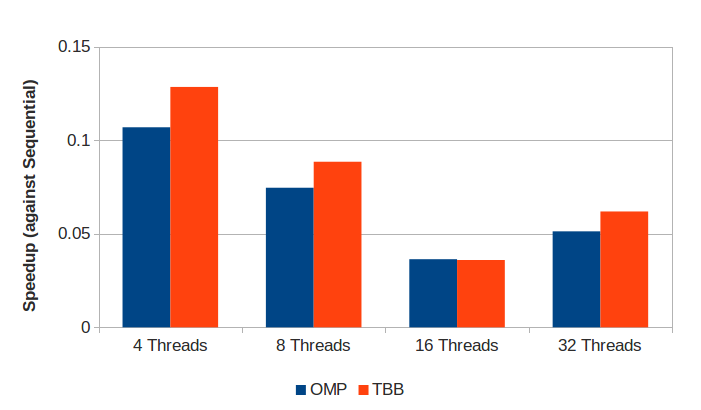
\includegraphics[width=\columnwidth]{plot-both-small}
	\caption{OpenMP vs TBB comparison on the smallest test case}
	\label{fig:both-small}
\end{figure}

\begin{figure}[!htp]
	\centering
	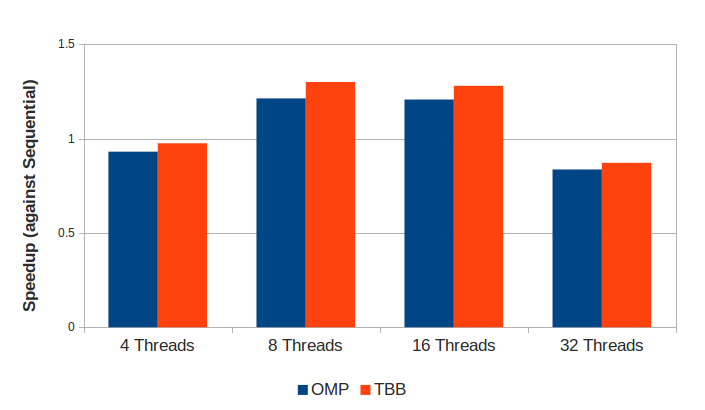
\includegraphics[width=\columnwidth]{plot-both-big}
	\caption{OpenMP vs TBB comparison on the largest test case}
	\label{fig:both-big}
\end{figure}

\Cref{fig:both-small} shows the speedup of each one for the smallest test case ($2^{11}$ keys) and \cref{fig:both-big} for the biggest test case ($2^{27}$ keys). In both cases, and also in the intermidiate ones that are not shown in this document, TBB managed to provide better speedups.

With a better parallel implementation, it could be possible that this small difference in speedup could escalate to a larger difference, but there was no way to prove that with the current implementation.
	\section{Conclusions}
\label{sec:900}

\todonaps{GET THIS DONE}
As for the programming approaches required by each of the two shared memory parallel libraries, it can be said that TBB, while providing excellent facilities to parallelize tasks and organize workload, also suffers from a couple of problems due to the paradigm it attempts to implement. Drawing much from functional paradigms, it requires the parallelizable logic to be encapsulated in a class object (namely, a \textit{Functor}). While this is good from a more abstract point of view, it also requires much more code to be written, for tasks that are sometimes rather simple. This issue might be solved with the usage of C++11 (recenlty known as C++0x), which allows the declaration of lambda functions. TBB supports this functions, allowing them to be passed as parameter to the parallelization directives, instead of an instance of a \textit{Functor}.

Another point that might provide some pitfalls to TBB is the complete abstraction of the threading model. While it is usually good to let the library handle all the background tasks of allocating threads and distribute the workload, this is not always the case. For most tasks it also possible to parameterize TBB functions, for example, with information about the desired granularity, which is useful to have some degree of control about the degree of division of the task.

It is not possible however, to have more low-level control over this. A particular example was found during the implementation of Radix Sort. Having each thread handling a set of buckets, with the index of those buckets being received as the chunck list to each thread, it was required to decide, for each element, wether or not the current thread was the one responsible for saving it. In OpenMP, this simply meant acquiring the thread id with the appropriate number, and decide from there if the destiny bucket was being handled by the current thread.
In TBB, however, there is no such thing as a thread id. This makes sense, but only to a certain extent, since it is TBB who decides how many threads are spawned. The only possible control over this is the maximum number of threads, but never the actual exact amount can be specified.
Because of this, the only way to determine if the bucket was assigned to the current thread was, for each element to insert, iterate over the entire chunck list, and check wether or not the index was there. This changed this computation from a simple bitwise operation and a comparison in OpenMP, to an entire loop in TBB

Even though the chunck is probably small enough to eliminate any performance issues from this difference, the fact remains that the lack of a more controlable parallelization feature hurt this version.

	\nocite*
	\bibliographystyle{cell}
	\bibliography{references}

\end{document}
